\begin{frame}[allowframebreaks]{Learning Autoregressive Models}
\begin{itemize}
    \item The goal of learning is to return a model $\hat{\mathcal{M}}$ that precisely captures the distribution $\mathcal{P}_{data}$ from which our data was sampled
    \item This is in general not achievable because of
    \begin{itemize}
        \item limited data only provides a rough approximation of the true underlying distribution
        \item computational reasons
    \end{itemize}
    \item Example. Suppose we represent each MNIST digit with a vector $\mathbf{X}$ of 784 binary variables (black vs. white pixel). How many possible states (= possible images) in the model? $2^{784} \approx 10^{236}$ . Even $10^7$ training examples provide extremely sparse coverage!
    \item We want to select $\hat{\mathcal{M}}$ to construct the ”best” approximation to the underlying distribution $\mathcal{P}_{data}$


\end{itemize}

\framebreak

\begin{itemize}
    \item We want to learn the full distribution so that later we can answer any probabilistic inference query
    \item We want to construct $\mathcal{P}_{\theta}$ as ”close” as possible to $\mathcal{P}_{data}$ (recall we assume we are given a dataset $\mathcal{D}$ of samples from $\mathcal{P}_{data}$)
    \begin{figure}
        \centering
        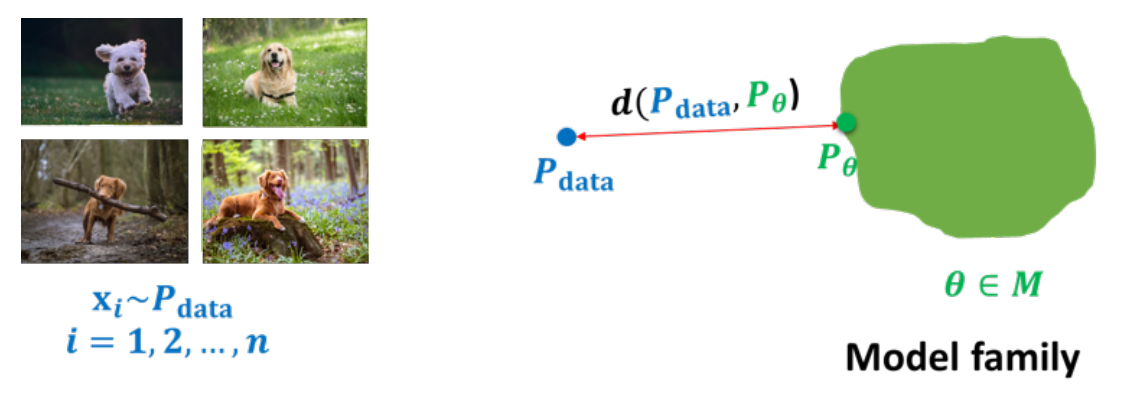
\includegraphics[height=1.3in]{images/autoregressive/learning.png}
        \caption*{Learning a generative model. $d(\cdot)$ is a distance measure.}
    \end{figure}
    
\end{itemize}
\end{frame}

\begin{frame}[allowframebreaks]{KL Divergence}
    \begin{itemize}
        \item How do we evaluate ”closeness” between model and data distribution?
        \item \textbf{Kullback-Leibler divergence} (KL-divergence) is one possibility:
        $$D(\mathcal{P}_{data}||\mathcal{P}_{\theta}) = E_{x \sim \mathcal{P}_{data}}   \left [log \left ( \frac{\mathcal{P}_{data}(x)}{\mathcal{P}_{\theta}(x)} \right ) \right ] = \sum_{x} \mathcal{P}_{data}(x) log \frac{\mathcal{P}_{data}(x)}{\mathcal{P}_{\theta}(x)}$$
        \item $D(\mathcal{P}_{data}||\mathcal{P}_{\theta})$ iff the two distributions are the same.
        \item It measures the ”compression loss” (in bits) of using $\mathcal{P}_{\theta}$ instead of $\mathcal{P}_{data}$.
    \end{itemize}
\end{frame}

\begin{frame}{Expected Log-Likelihood}

\begin{itemize}
    \item We can simplify this somewhat:
    \begin{equation}
    \begin{split}
        D(\mathcal{P}_{data}||\mathcal{P}_{\theta}) & = E_{x \sim \mathcal{P}_{data}}   \left [log \left ( \frac{\mathcal{P}_{data}(x)}{\mathcal{P}_{\theta}(x)} \right ) \right ] \\
         & = E_{x \sim \mathcal{P}_{data}} [log \mathcal{P}_{data}(x)] - E_{x \sim \mathcal{P}_{data}} [log \mathcal{P}_{\theta}(x)]
    \end{split}
    \end{equation}
    
    \item The first term does not depend on $\mathcal{P}_{\theta}$. Then, \emph{minimizing} KL divergence is equivalent to \emph{maximizing} the \textbf{expected log-likelihood}
    \begin{equation}
    \begin{split}
        \arg\min_{\mathcal{P}_{\theta}} D(\mathcal{P}_{data}||\mathcal{P}_{\theta}) & = \arg\min_{\mathcal{P}_{\theta}} - E_{x \sim \mathcal{P}_{data}} [log \mathcal{P}_{\theta}(x)]\\
        & = \arg\max_{\mathcal{P}_{\theta}} E_{x \sim \mathcal{P}_{data}} [log \mathcal{P}_{\theta}(x)]
    \end{split}
    \end{equation}
    
    \begin{itemize}
        \item Asks that $\mathcal{P}_{\theta}$ assign high probability to instances sampled from $\mathcal{P}_{data}$, so as to reflect the true distribution
        \item Because of log, samples $x$ where $\mathcal{P}_{\theta}(x) \approx 0$ weigh heavily in objective

    \end{itemize}
    \item Although we can now compare models, since we are ignoring $H(\mathcal{P}_{data})$, we don’t know how close we are to the optimum.
    \item Problem: In general we do not know $\mathcal{P}_{data}$

\end{itemize}
\end{frame}

\begin{frame}{Maximum Likelihood}
\begin{itemize}
    \item Approximate the expected log-likelihood
    $$ E_{x \sim \mathcal{P}_{data}} [log \mathcal{P}_{\theta}(x)]$$
    with the empirical log-likelihood:
    $$E_{\mathcal{D}} = \frac{1}{\mathcal{D}} \sum_{x \in \mathcal{D}} log \mathcal{P}_{\theta}(x)$$
    \item \textbf{Maximum likelihood learning} is then:
        $$\arg\max_{\mathcal{P}_{\theta}} \frac{1}{\mathcal{D}} \sum_{x \in \mathcal{D}} log \mathcal{P}_{\theta}(x)$$
\end{itemize}
\end{frame}

\begin{frame}[allowframebreaks]{Recurrent Neural Networks (RNN)}
\begin{itemize}
    \item The next form of autoregressive models
    \item \textbf{Challenge}: model $\mathcal{P}(x_t|x_{1:t-1}; \alpha^t)$. "History" $x_{1:t-1}$ keeps getting longer.
    \item \textbf{Idea}:  keep a summary and recursively update it
    \end{itemize}
    % \begin{figure}
    %     \centering
    %     \includegraphics[height=1.3in]{./images/rnn.PNG}
    %     \caption*{Recurrent Neural Network (RNN) samaple architecture.}
    % \end{figure}
    % \item Hidden layer $h_t$ is a summary of the inputs seen till time $t$

\framebreak
\begin{figure}
    \centering
    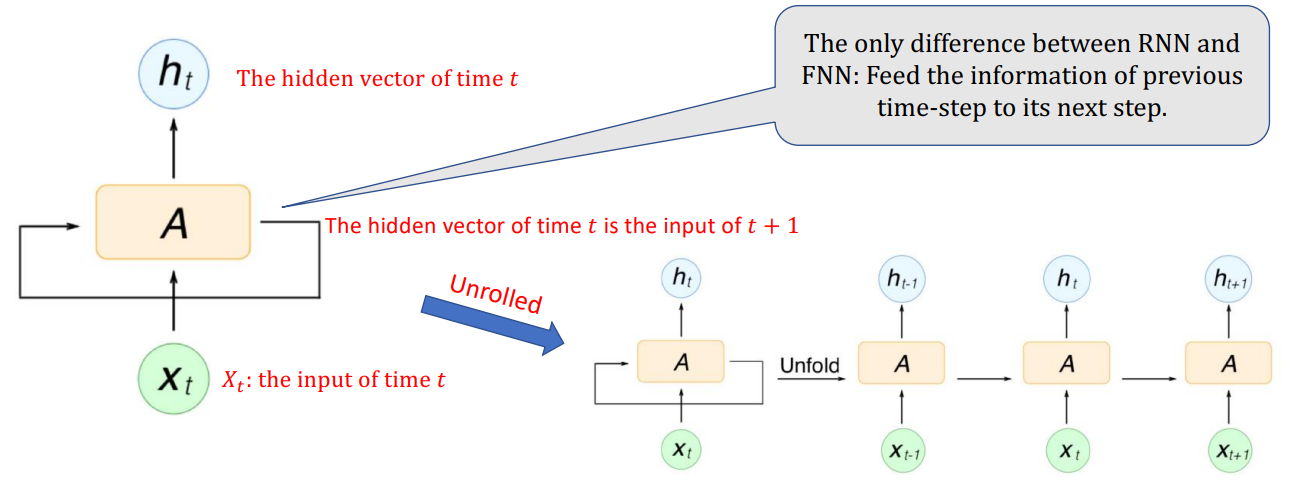
\includegraphics[height=0.9\textheight, width=\textwidth, keepaspectratio]{images/autoregressive/rnn_2.png}
    \caption*{Recurrent Neural Network (RNN) sample architecture.}
\end{figure}

\framebreak
Pros:
\begin{itemize}
    \item Can be applied to sequences of arbitrary length.
    \item Very general: For every computable function, there exists a finite RNN that can compute it
\end{itemize}
\vskip 10pt
Cons:
\begin{itemize}
    \item Still requires an ordering
    \item Sequential likelihood evaluation (very slow for training)
    \item Sequential generation (unavoidable in an autoregressive model)
    \item Can be difficult to train (vanishing/exploding gradients)
\end{itemize}
\end{frame}

\begin{frame}{RNNs}

\framebreak
\begin{figure}
    \centering
    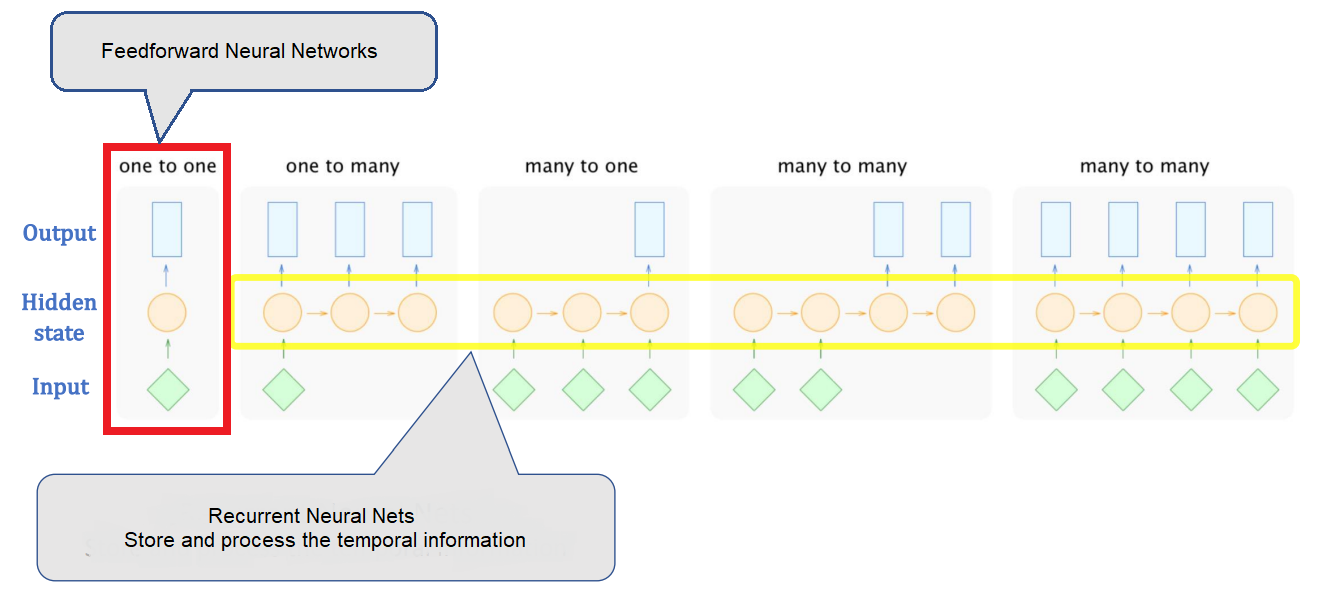
\includegraphics[height=0.9\textheight, width=\textwidth, keepaspectratio]{images/autoregressive/rnn_types.png}
    \caption*{Different sequential modeling types}
\end{figure}
    
\end{frame}

\begin{frame}[allowframebreaks]{RNNs - Examples}
\textbf{Image Captioning}
\begin{figure}
    \centering
    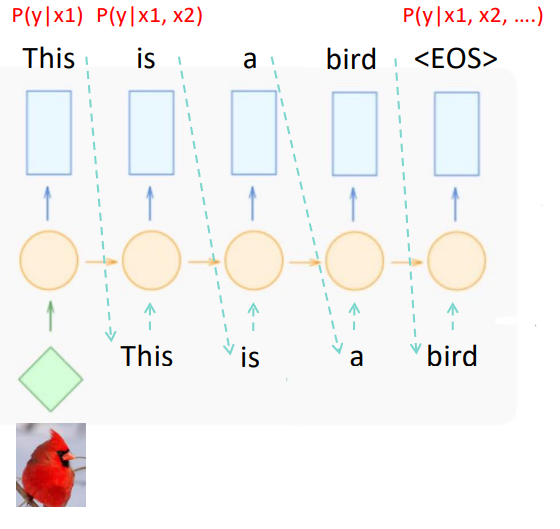
\includegraphics[height=0.7\textheight, width=\textwidth, keepaspectratio]{images/autoregressive/image_cap.png}
    \caption*{Image captioning with RNNs}
\end{figure}

\framebreak
\textbf{Text Generation}
\begin{figure}
    \centering
    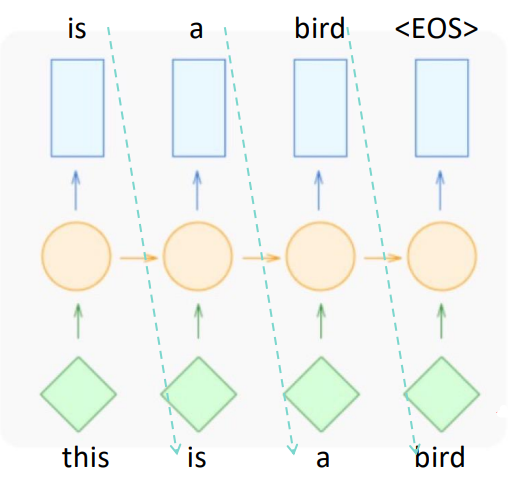
\includegraphics[height=0.7\textheight, width=\textwidth, keepaspectratio]{images/autoregressive/text_gen_ex.png}
    \caption*{Text generation with RNNs}
\end{figure}

\framebreak
\textbf{Chatbot}
\begin{figure}
    \centering
    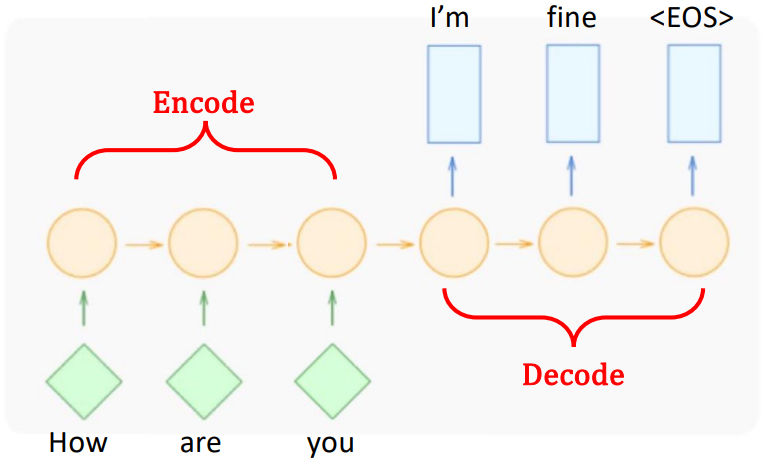
\includegraphics[height=0.7\textheight, width=\textwidth, keepaspectratio]{images/autoregressive/chatbot.png}
    \caption*{Chatbot with RNNs}
\end{figure}
\end{frame}